%%
%% This is file `sample-sigconf.tex',
%% generated with the docstrip utility.
%%
%% The original source files were:
%%
%% samples.dtx  (with options: `sigconf')
%% 
%% IMPORTANT NOTICE:
%% 
%% For the copyright see the source file.
%% 
%% Any modified versions of this file must be renamed
%% with new filenames distinct from sample-sigconf.tex.
%% 
%% For distribution of the original source see the terms
%% for copying and modification in the file samples.dtx.
%% 
%% This generated file may be distributed as long as the
%% original source files, as listed above, are part of the
%% same distribution. (The sources need not necessarily be
%% in the same archive or directory.)
%%
%% The first command in your LaTeX source must be the \documentclass command.
\documentclass[sigconf,nonacm=true]{acmart}
\usepackage{listings}
\usepackage{booktabs}% More proffesional look of tables.
\usepackage{siunitx}% An awesome package for typesetting and manipulation numbers and units.
\usepackage{caption}% Better control over caption
\usepackage{lipsum}% Example text
\usepackage{xcolor}
\usepackage{hyperref}
\usepackage{adjustbox}
\hypersetup{
	colorlinks=true,
	linkcolor=blue,
	filecolor=magenta,      
	urlcolor=cyan,
}


\pagecolor{white}
\lstset{
basicstyle=\ttfamily,
frame=single
}
%%
%% \BibTeX command to typeset BibTeX logo in the docs
\AtBeginDocument{%
  \providecommand\BibTeX{{%
    \normalfont B\kern-0.5em{\scshape i\kern-0.25em b}\kern-0.8em\TeX}}}

%% Rights management information.  This information is sent to you
%% when you complete the rights form.  These commands have SAMPLE
%% values in them; it is your responsibility as an author to replace
%% the commands and values with those provided to you when you
%% complete the rights form.
\setcopyright{none}
%%\copyrightyear{2020}
%%\acmYear{2020}
%%\acmDOI{10.1145/1122445.1122456}

%% These commands are for a PROCEEDINGS abstract or paper.
%% \acmConference[Woodstock '18]{Woodstock '18: ACM Symposium on Neural
%%   Gaze Detection}{June 03--05, 2018}{Woodstock, NY}
%% \acmBooktitle{Woodstock '18: ACM Symposium on Neural Gaze Detection,
%%   June 03--05, 2018, Woodstock, NY}
%% \acmPrice{15.00}
%% \acmISBN{978-1-4503-XXXX-X/18/06}


%%
%% Submission ID.
%% Use this when submitting an article to a sponsored event. You'll
%% receive a unique submission ID from the organizers
%% of the event, and this ID should be used as the parameter to this command.
%%\acmSubmissionID{123-A56-BU3}

%%
%% The majority of ACM publications use numbered citations and
%% references.  The command \citestyle{authoryear} switches to the
%% "author year" style.
%%
%% If you are preparing content for an event
%% sponsored by ACM SIGGRAPH, you must use the "author year" style of
%% citations and references.
%% Uncommenting
%% the next command will enable that style.
%%\citestyle{acmauthoryear}

%%
%% end of the preamble, start of the body of the document source.
\begin{document}

%%
%% The "title" command has an optional parameter,
%% allowing the author to define a "short title" to be used in page headers.
\title{CE/CZ4045 Assignment Part 1}

%%
%% The "author" command and its associated commands are used to define
%% the authors and their affiliations.
%% Of note is the shared affiliation of the first two authors, and the
%% "authornote" and "authornotemark" commands
%% used to denote shared contribution to the research.

\author{Lim Jun Hong}
\affiliation{\institution{Nanyang Technological University}}
\email{LIMJ0209@e.ntu.edu.sg}

\author{Tammy Lim Lee Xin}
\affiliation{\institution{Nanyang Technological University}}
\email{TLIM045@e.ntu.edu.sg}

\author{Lee Han Wei}
\affiliation{\institution{Nanyang Technological University}}
\email{B160017@e.ntu.edu.sg}

\author{Pang Yu Shao}
\affiliation{\institution{Nanyang Technological University}}
\email{C170134@e.ntu.edu.sg}

%%
%% By default, the full list of authors will be used in the page
%% headers. Often, this list is too long, and will overlap
%% other information printed in the page headers. This command allows
%% the author to define a more concise list
%% of authors' names for this purpose.
%% \renewcommand{\shortauthors}{Trovato and Tobin, et al.}

%%
%% The abstract is a short summary of the work to be presented in the
%% article.


%%
%% Keywords. The author(s) should pick words that accurately describe
%% the work being presented. Separate the keywords with commas.
%% \keywords{NLP, Text Tagging, Information Retreival}

%% A "teaser" image appears between the author and affiliation
%% information and the body of the document, and typically spans the
%% page.

%% \begin{teaserfigure}
%%   \includegraphics[width=\textwidth]{sampleteaser}
%%   \caption{Seattle Mariners at Spring Training, 2010.}
%%   \Description{Enjoying the baseball game from the third-base
%%   seats. Ichiro Suzuki preparing to bat.}
%%   \label{fig:teaser}
%% \end{teaserfigure}

%%
%% This command processes the author and affiliation and title
%% information and builds the first part of the formatted document.
\maketitle

\section{Introduction}
In this assignment, we first perform domain specific data analysis by comparing the effectiveness of applying the various NLP processes (e.g. Tokenizing, Stemming, Segmentation, POS Tagging) to texts belonging in different domains. 

Next, using a separate dataset of reviews of a product/service, we identify <Noun-Adjective> pairs manually and programmatically and rank them. The results of the ranking produced by ourselves and the program is then compared and analysed. 

Lastly, using the same dataset of reviews, a NLP application is developed. The implementation of all tasks will be discussed in detail in the following sections.

For implementing the various parts of this assignment, the following external Python libraries are used:
\begin{itemize}
	\item NLTK
	\item SpaCy
	\item pandas
	\item scikit-learn
\end{itemize}

\section{Domain Specific Dataset Analysis}
The 3 datasets chosen for analysis are from different domain specific Reddit forums:
\begin{itemize}
	\item {\verb|Investments|}: r/wallstreetbets
	\item {\verb|Mechanical Keyboards|}: r/mechanicalkeyboards
	\item {\verb|Programming|}: r/programming
\end{itemize}

\subsection{Tokenization} 
The NLTK function \textit{word\_tokenize()} was used to tokenize each comment. This function splits tokens based on white space and punctuation. Figure 1 shows the function being implemented in our code and Figure 2 shows the resulting tokens after running the tokenizer function on a single comment. \bigskip

\renewcommand{\lstlistingname}{Figure}% Listing -> Algorithm
\renewcommand{\lstlistlistingname}{List of \lstlistingname s}% List of Listings -> List of Algorithms

\begin{figure}[H]
	\begin{lstlisting}[gobble=10]
	    w = nltk.word_tokenize(comment.body)
	    wsb_words.extend(w)
	    count+=1
	    print("Comment:", comment.body)
	\end{lstlisting}
	\caption{Implementation of Tokenizer}
\end{figure}

\begin{figure}[H]
	\begin{lstlisting}[gobble=10]
	    Comment: Tesla calls!
	    Token results: ['Tesla', 'calls', '!']
	\end{lstlisting}
	\caption{Result of Tokenizer}
\end{figure}

\subsection{Evaluation of tokenizer results}
The tokenizer was successful in tokenizing most data in the chosen dataset. However, upon manual inspection of each tokenized result, we found some incorrect tokens as shown in Table~\ref{tab:token}. The incorrect tokens were mainly due to domain specific issues. For instance, in r/programming, the tokenizer incorrectly tokenized a line of code and separated the code into three tokens instead of one. Another common error is due to the separation of domain specific terminologies such as investment terms like “options flow” and names of mechanical switches like “Holy Pandas”.

\begin{table}[h]
	\begin{tabular}{|l|l|}
	\hline
	 {\bf Expected Token} &  {\bf Actual token} \\ \hline
	 “Martin Luther King”& “Martin”, ”Luther”, ”King”  \\ \hline
	 “Options flow” &  “Options”,”flow” \\ \hline
	 “Holy Pandas”& “Holy”, ”Pandas” \\ \hline
	“:)” &  “:”, “)”\\ \hline
	 “System.nanoTime()”& “System.nanoTime”, “(“,”)” \\ \hline
	“String Buffer:”, “1 ms”  &  “String Buffer:1”, “ms”\\ \hline
	\end{tabular}
	\caption{Incorrectly identified tokens}
	\label{tab:token}
\end{table}


\subsection{Methods to improve tokenizer}
Based on the results shown in the table above, the tokenizer could be further improved by implementing the following methods. \medskip


{\bf Context specific tokens}
The dataset used in this assignment is from an online forum, Reddit. As such, many informal tokens such as emojis are used but the current tokenizer is unable to tokenize it correctly. For example, “:)” will be tokenized into 2 tokens, “:” and “)” which loses its meaning. Tokenizers such as TweetTokenizer are able to recognize such tokens.\bigskip

 {\bf Multi-word expressions:}
To prevent the tokenizer from splitting multi-word expressions, a function such as the NLTK MWETokenizer could be implemented. This function takes a string that has been divided into tokens and re\-tokenize it by merging into a multi-word expression. For example, the tokens “ Martin” ,”Luther”, “King” will be re\-tokenized into a single token, “Martin Luther King”. \smallskip

 {\bf Regular expressions:}
Regular expressions could also be used to ensure sequences such as money expressions and percentage expressions are tokenized as a singular token. For example, currently word\_tokenizer tokenizes the word “60\%” to 2 separate tokens, “60” and “\%” although it is more meaningful to have it as a single token which could be done by regular expression. 



\subsection{Stemming}
After getting the word tokens for each comment, the NLTK function porterStemmer() is used to reduce each word token to its root or base by removing common morphological and inflexional token endings.

To ensure that the data used for plotting of token distribution would be meaningful, we added a list of stop words which are words that do not contribute to a deeper meaning for the analysis. Such words include common punctuations such as commas and fullstops. \linebreak
\begin{figure}
	\centering
	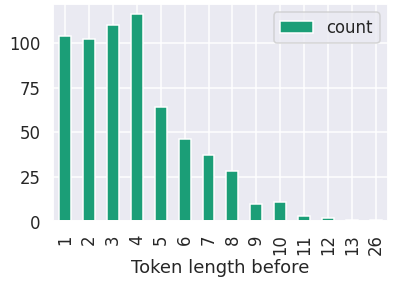
\includegraphics[scale=0.55]{ss1.png}
	\caption{Token length before stemming}
\end{figure}


\begin{figure}[H]
    \centering
    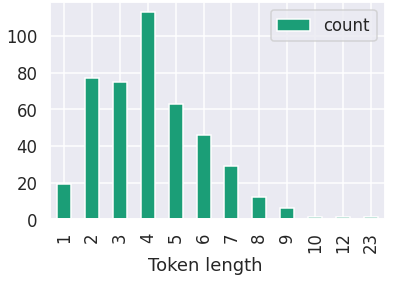
\includegraphics[scale=0.55]{ss2.png}
   	\caption{Token length after stemming}
\end{figure}
The distribution graphs above shows that most tokens have 4 number of characters. Prior to stemming, the upper range for length is from 10 to 26 number of characters. After stemming, this upper range significantly decreased to 7 to 9 number of characters. This is due to the process of stemming reducing common token endings, which thus translates into a lower number of characters. 

\subsection{Sentence Segmentation}
The NLTK function \textit{sent\_tokenize()} uses an instance of \textit{PunktSentenceTokenizer} from the \textit{nltk.tokenize.punkt} module which has already been trained and knows very well where to mark the end and beginning of a sentence at what characters and punctuation. \smallskip

\begin{figure}[H]
	\centering
	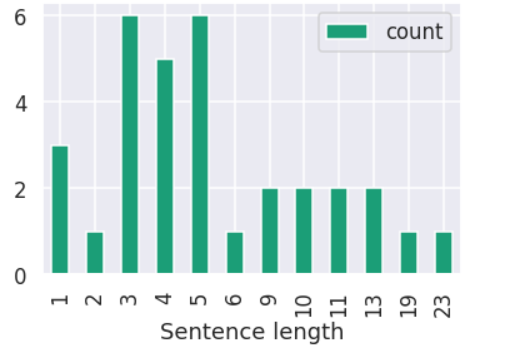
\includegraphics[scale = 0.35]{sentence1.png}
	\caption{Wallstreetbets}
\end{figure}
\begin{figure}[H]
	\centering
	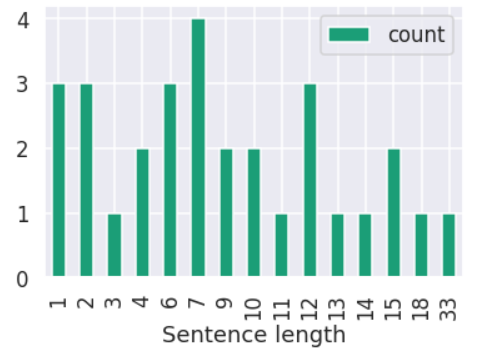
\includegraphics[scale=0.35]{sentence2.png}
	\caption{Mechanicalkeyboards}
\end{figure}
\begin{figure}[H]
	\centering
	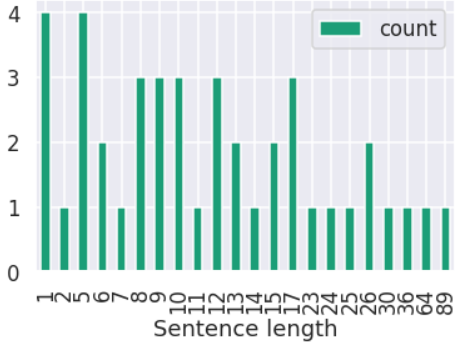
\includegraphics[scale=0.35]{sentence3.png}
	\caption{Programming}
\end{figure}
From the graph of 20 sentences being sampled from each domain, we can see the difference in the sentence length between the different domains. ‘Wallstreetbets’ is a community mainly focused on the U.S. stock market, ‘mechanicalkeyboards’ is a community where people would post images about their own mechanical keyboards or seek for recommendations of parts or mechanical keyboards to purchase and lastly, ‘programming’ is a community where programmers would be there to discuss about programming related question or the uses of different languages. \smallskip

For ‘wallstreetbets’, the majority of the sentences are about 3-5 words long which is common in Reddit where people just leave comments about what they think. The comments usually reflect the reaction of a news article posted about the U.S. stock market thus the sentences aren’t that long. As compared to ‘mechanicalkeyboards’, the sentences are much longer, where people would be curious about the parts used in the mechanical keyboard posted or queries from commenters about the experience with the mechanical keyboard. ‘Programming’ in reddit has the widest range of sentence length in answer because of the nature of the subreddit. With more questions and elaborated answers, we can tell from Figure 2.3 that there are very long sentences as compared to ‘wallstreetbets’ and ‘mechanicalkeyboards’ causing a wide spectrum in length of the sentences.
\subsection{Part-Of-Speech Tagging(POS Tagging)}
The NLTK function \textit{nltk.pos\_tag()} takes a string and tags the words in the string to their respective POS tags. \textit{nltk.pos\_tag()} is a machine-learning tagger that has been well-trained by Microsoft and the model is saved for people to use. Since there are no perfect taggers around, there were definitely some errors made by the tagger especially when it comes to domain-specific terms.

For ‘wallstreetbets’, from one of the randomly selected comments, ‘hexo’ was tagged as NN instead of NNP, a proper noun when it is a name for a U.S. stock, Hexo Corp. ‘gme’ was incorrectly tagged as NN instead of a proper noun because ‘gme’ meant GameStop Corp. in the context of ‘wallstreetbets’.

For ‘mechanicalkeyboards’, there are words that are incorrectly tagged too. There are many different keyboard switches that are named by their brands. One of the comments had ‘alpaca/’, ‘tangerine’ and ‘switches’ tagged as adjective, noun, and plural nouns respectively when these 3 words are supposed to be tagged as a proper noun. Domain-specific words are not identified correctly due to the limitation of the NLTK library.

For ‘programming’, there are still technical roles in the infocomm technology that are tagged incorrectly. ‘System admins’ are tagged separately by NLTK when it is a role in the office. Some commonly used programming terms such as ‘print’ and ‘i-o’ also known as input output are technical terms used in the programming syntax but are tagged as adjectives by NLTK.

From the results of 3 different domains, we can see that NLTK POS tagging system is not perfect, however there is no perfect tagging system for all the domains. The results are as expected even though NLTK’s machine learning model is often being updated by the open-source community. If the POS Tagging system is not trained with the correct corpus or edited by the programmers, domain specific terms would highly likely be identified incorrectly.

\section{Development of a <Noun - Adjective> Pair Ranker}
In this section, a <Noun-Adjective> pair ranker is developed to identify the top 5 meaningful pairs. 

First, the top 5 meaningful pairs is identified manually and then a ranker will be implemented using Python to do it programmatically. 

Next, the differences between the results of the manually identified pairs as well as those returned by the program is compared. 

Lastly, the potential challenges that may be encountered during the language processing process is discussed.

\subsection{Methodology and Tools}
The <Noun-Adjective> pairs are ranked in accordance to their \textbf{Occurrence Count} (i.e., a pair with the most occurrences will be the top ranked pair).

\subsubsection{Manual Identification}
Manual Identification is done based on the user's knowledge of vocabulary as well as the user's interpretation. The user will classify the pairs according to the definition after two words are paired with one another. There is a possibility whereby different word pairs might convey similar meanings (e.g., tall waterfall, highest waterfall, etc.).
\subsubsection{Python-based NLP Library}
The library \verb|SpaCy| is chosen for the implementation of the <Noun - Adjective> pair ranking program as \verb|SpaCy| is one of the newer libraries implemented in Python for NLP tasks as compared to older libraries such as \verb|NLTK|. It also has performance benefits as it uses latest algorithms for tasks such as syntax parsing, making it faster than \verb|NLTK| for many text processing tasks.

\subsection{Dataset}
\label{subsection:dataset}
The dataset used for this task as well as for the NLP application developed in Section \ref{section:label} is the collection of reviews of \textbf{Jewel Changi Airport} on \href{https://www.tripadvisor.com.sg/Attraction_Review-g294265-d17237163-Reviews-Jewel_Changi_Airport-Singapore.html}{Tripadvisor}

A web-scraper was developed to scrape the reviews which is then stored locally as a .csv file which can be easily read by the implemented programs.

\subsection{Results}
\subsubsection{Manually Identified Pairs Ranking}
By identifying the <Noun-Adjectives> pairs manually, the following results are obtained:
\begin{table}[H]
	\label{tab:manualpairs}
	\begin{adjustbox}{width=\columnwidth}
	\begin{tabular}{ccc}
		\toprule
		Noun&Adjective&Occurrence Count\\
		\midrule
		waterfall & amazing/great/marvelous/spectacular & 6 \\
		waterfall & tallest/biggest & 4 \\
		place & amazing/good/extraordinary & 4 \\
		airport & beautiful & 2 \\
		airport & amazing/impressive & 2 \\
		\bottomrule
	\end{tabular}
	\end{adjustbox}
	\caption{Top 5 <Noun-Adjective> Pairs Identified Manually}
\end{table}


\subsubsection{Programmatically Identified Pairs Ranking}
By using the implemented Python script to identify the <Noun-Adjectives> pairs, the following results are obtained:
\begin{table}[H]
	\label{tab:progpairs}
	\begin{tabular}{ccc}
		\toprule
		Noun&Adjective&Occurrence Count\\
		\midrule
		waterfall & indoor & 6 \\
		floor & top & 2 \\
		place & amazing & 2 \\
		level & new & 2 \\
		level & top & 2 \\
		\bottomrule
	\end{tabular}
	\caption{Top 5 <Noun-Adjective> Pairs Identified by Program}
\end{table}

\subsection{Analysis}
We identified that the output from the SpaCy text processing does not accurately reflect how the users think about the Jewel airport. \textbf{4} out of \textbf{5} <noun> – <adjective> pairs  (indoor waterfall, top floor, new level and top level) are referring to an object without further clarification of how the users view it.  One of the main challenges in this exercise was POS tagging as a word can have multiple tags. At the same time, different word combinations can imply the same meaning and the library is unable to group them together.

Among the manually extracted <noun> – <adjective> pairs, the noun <waterwall> is the most common and users often describe it as <waterfall>- <biggest>. The other common nouns are <place> and <airport> where the users often describe it with different adjectives of similar meaning. Having a manual categorization helps to gather similar terms under one umbrella instead of separating the counts.

A possible improvement to the implemented program is to use a \textbf{thesaurus} to group "similar" words into a single category, this would then be able overcome the previously identified problem where the program would classify these similar pairs as separate counts rather than counting them together. However, it is worth noting that the thesaurus is also limited by the corpus which it is developed upon. In specialized domains, a generic thesaurus might not be sufficient and for those instances human intervention might still be necessary.


\section{Application: Search Engine}
\label{section:label}
Based on the reviews collected in section \ref{subsection:dataset}, A simple search
engine is developed which allows the user to search for related reviews
based on the user's input.

With the user's input (i.e., the search query), the list
of relevant reviews is retrieved and the reviews are ranked according
to their similarity, which is presented in descending order to the user.

\subsection{Implementation}
The application is implemented using \verb|Python 3.7.9| with the following external
libraries:
\begin{itemize}
	\item {\verb|pandas|}: For general DataFrame processing
	\item {\verb|scikit-learn|}: For calculating tf-idf / cosine similarity
\end{itemize}


\subsection{TF-IDF Vectorization of Reviews}
For implementing the search engine, the reviews must first be represented by
\verb|tf-idf| vectors instead of plain-text. This will allow the computation
of the similarity between the document/review vector and the query vector.

To generate the \verb|tf-idf| vectors, every review is first preprocessed by 
case-folding, removing stopwords and tokenized to generate a 
\textbf{Bag of Words} representation. The term counts are used to generate the
\verb|tf-idf| values.
\begin{itemize}
	\item \textbf{Term Frequency} (\verb|tf|), is a measure of how often a term occurs
	in the document.
	\item \textbf{Inverse Document Frequency} (\verb|idf|), is a measure of how much
	information the term provides (i.e., how rare the term is) across
	\textbf{all documents}.
\end{itemize}
The \verb|scikit-learn| library provides a module,
\begin{verbatim}
	sklearn.feature_extraction.text.TfidfVectorizer
\end{verbatim}
which automatically performs basic preprocessing of the text mentioned above and
transforms the array of documents into a tf-idf vector while also performing some
normalizing and smoothing to the data.


\subsection{Querying and Ranking Reviews}
A Search Engine is required to take in a user's query and display \textit{relevant} 
documents to the user. Since tf-idf vectors have already been built for the 
existing documents (reviews), the user's query can be transformed to a tf-idf vector
as well and the similarity can be computed based on some similarity measure.

\verb|TfidfVectorizer| also provides a method \verb|transform|, which builds a tf-idf
vector from a document based on the Language Model that it has learned. With both the
query and documents represented in \verb|tf-idf| vectors, the similarity between the
query vector and all document vectors can be computed. A few distance measures that
can be used include:

\begin{itemize}
	\item Manhattan Distance
	\item Euclidean Distance
	\item Cosine Similarity
\end{itemize}

For our search application, the \textbf{Cosine Similarity} measure is used.
Search queries have a short length in nature, therefore using Manhattan / 
Euclidean distance could cause a potential document of interest have a large
distance (i.e., appear dissimilar) when compared to the query. For instance,
consider the example vocabulary in Table~\ref{tab:vocab} and the following
documents and query:

\begin{itemize}
	\item Document 1: apple apple apple apple apple apple 
	\item Document 2: banana orange
	\item Query: apple
\end{itemize}
These would yield the following term count vectors:
\begin{displaymath}
	D1 = \begin{pmatrix}6 & 0 & 0\end{pmatrix}
\end{displaymath}
\begin{displaymath}
	D2 = \begin{pmatrix}0 & 1 & 1\end{pmatrix}
\end{displaymath}
\begin{displaymath}
	Q = \begin{pmatrix}1 & 0 & 0\end{pmatrix}
\end{displaymath}
By calculating the euclidean distance between the query and the documents,
the following Euclidean distances are obtained:
\begin{displaymath}
	Euclidean(D1,Q) = 5
\end{displaymath}
\begin{displaymath}
	Euclidean(D2,Q) = 1.732
\end{displaymath}
Here, the distance between D2 and Q is smaller than that of the distance
between D1 and Q, however it can be observed by D1 should be the more similar
document. Therefore, it can be concluded that measures such as Manhattan and
Euclidean distances can be affected by the magnitude of the vector, even when
both the query and the document vectors share similar components.

The Cosine Similarity overcomes this as it is a measure of the \textit{angle}
between two vectors. As search queries are short in nature, it is able to retrieve
documents which share similar components to the query vector.

\begin{table}
	\begin{tabular}{ccl}
		\toprule
		Word Id&Word\\
		\midrule
		0 & apple\\
		1 & banana\\
		2 & orange\\
		\bottomrule
	\end{tabular}
	\caption{Example Vocabulary}
	\label{tab:vocab}
\end{table}


\subsection{Application Demo}
A sample run of the application is shown below:
\begin{lstlisting}
Reviews 1 to 5 (out of 167) for search query 
"Fountain light show"
=============================================

1: The Jewel is the gigantic shopping mall 
with varieties of shops and restaurants. 
The famous one is the fountain that shall 
make you stop to see it.  At night time there
are the light show at Fountain.

Recommend for visiting

2: This has to be seen to be believed. 
Gardens, waterfalls, restaurants, shops, 
adventure park and monorail. Allow at least 
a few hours here and stay for light show. 
Light show not great but colored waterfall 
is impressive. A must see.

. . .
\end{lstlisting}

\newpage
\section{Conclusion}
In this assignment, we have successfully implemented various NLP processes that has been taught to us in the first-half of the course such as
\begin{itemize}
	\item Tokenization
	\item Stemming
	\item Sentence Segmentation
	\item POS Tagging
\end{itemize}
The effectiveness of these algorithms on specialized texts has also been explored and evaluated.

In the second section, we have also performed analysis of <Noun-Adjective> pairs on a \textbf{"practical"} dataset of reviews on Jewel Changi Airport and discussed the limitations of the NLP algorithms and instances where human intervention or interpretation of data might still be necessary. 

Lastly, we have implemented a NLP application in the form of a search engine which allows a user of the application to search for related reviews based on a query. The implementation considerations such as representation of the reviews/queries as well as the choice of similarity measure to be used when ranking reviews have been discussed as well.

After this assignment, we have a better appreciation of the various NLP techniques that were taught after being able to apply it in a practical manner as well as more familiarity with the various high-level Python libraries available which provides implementations of the various algorithms for NLP tasks.


\end{document}
\endinput
%%
%% End of file `sample-sigconf.tex'.
